\chapter{Laboratory observations of slow earthquakes\\ and the spectrum of tectonic fault slip modes}

\section{Abstract}
Slow earthquakes represent an important conundrum in earthquake physics. Whereas regular earthquakes are catastrophic events with rupture velocities governed by elastic wave speed, the processes that underlie slow fault slip phenomena, including recent discoveries of tremor, slow slip, and low frequency earthquakes, are less understood. Theoretical models and sparse laboratory observations have provided insights, but the physics of slow fault rupture remain enigmatic. Here we report on laboratory observations that illuminate the mechanics of slow slip phenomena.  We show that a spectrum of slow slip behaviors arise near the threshold between stable and unstable failure, and is governed by frictional dynamics via the interplay of fault frictional properties, effective normal stress, and the elastic stiffness of the surrounding material. This generalizable frictional mechanism may act in concert with other hypothesized processes that damp dynamic ruptures, and is consistent with the broad range of geologic environments where slow earthquakes are observed.

\section{Introduction}
Slow earthquakes are a mode of self-sustained fault rupture in which slip accelerates but does not reach rates sufficient to radiate high-frequency seismic energy\cite{linde1996san, obara2002nonvolcanic}. Seismic and geodetic observations reveal that slow slip and the related phenomena of low-frequency earthquakes and non-volcanic tremor define a spectrum of slip behaviors that unfold over timescales ranging from seconds to months\cite{obara2002nonvolcanic, rogers2003episodic, ide2007scaling, shelly2007non, peng2010integrated}. Slow earthquakes can be large, in some cases equivalent to M7+ earthquakes, and they may play a role in stress transfer and thus triggering of damaging regular earthquakes\cite{kato2012propagation}.  Slow earthquakes have also been observed as precursors to regular earthquakes and thus they may provide insight into the processes of earthquake nucleation\cite{houston2015low, hawthorne2010tidal}.  Although geophysical observations have resolved fine details of slow earthquake slip and propagation rates of tectonic fault tremor\cite{peng2010integrated,houston2015low,hawthorne2010tidal,shelly2010migrating}, the fundamental and controlling mechanics of these phenomena remain enigmatic. 

Regular earthquakes have long been understood in terms of stick-slip failure dictated by frictional and elastic properties of Earth's crust \cite{Brace_1966}. Laboratory studies have provided key insights into the physics of fault failure and its dynamics, both for repeating earthquake-like stick-slip failure and for more complex slip behaviors. For example, previous works have reported a range of observations including transient slip, oscillatory sliding behavior, and dynamic rupture at sub-Raleigh and supershear propagation speeds\cite{voisin2008evolution, shimamoto1986transition, baumberger1994crossover, kaproth2013slow, ben2010slip, passelegue2013sub, scholz1972detailed}.  Transient and oscillatory behavior have been interpreted as analogs for premonitory slip prior to earthquakes or transient aseismic slip \cite{voisin2008evolution, scholz1972detailed,rubin2011designer}.  

Despite their relevance to natural fault zones and slow earthquakes, detailed laboratory observations of repetitive slow slip transients are few and do not include systematic studies. These behaviors have been reported in some experimental work \cite{voisin2008evolution, baumberger1994crossover, kaproth2013slow}, but have been interpreted and modeled in the context of specific fault rheologies, using so-called 'designer` friction laws. In one form of these laws, slow stick-slip is produced by an increase in frictional resistance with slip velocity, such that instability is quenched during acceleration \cite{baumberger1994crossover, kaproth2013slow, rubin2011designer}.  Other explanations for slow earthquakes have focused on processes that may arrest slip acceleration during earthquake nucleation, including dilatancy hardening \cite{liu2007spontaneous,segall2010dilatant} transitional frictional behavior as a function of slip \cite{ikari2013slip} or slip rate, and fault zone heterogeneity.  Some numerical simulations successfully predict complex slip behavior, including oscillatory behavior and the emergence of periodic slow slip \cite{liu2007spontaneous,gu1984slip}. Two dimensional numerical models also show promise in reproducing natural events, with fewer free parameters than multiple state variable models26. 

To date, the origin of slow earthquakes has been explored largely via seismic or geodetic data or through numerical experiments with only sparse, isolated laboratory observations to probe the underlying mechanics.  Although theoretical models can explain the emergence of slow-slip transients under certain conditions or for specific frictional rheologies \cite{liu2007spontaneous,segall2010dilatant,gu1984slip}, a fundamental mechanical explanation for these events remains elusive. Yet, slow modes of fault rupture are observed in a variety of tectonic and geologic settings, and with a wide range of durations, raising the question as to whether they arise from a universal mechanism \cite{peng2010integrated,den2012new}. 

Although many fault zones are rich in phyllosilicate minerals, which have been shown to exhibit both rate-weakening and rate-strengthening behavior under conditions comparable to those expected in situ in the seismogenic crust \cite{ide2007mechanism, saffer2001laboratory, den2013influence}, we focus on quartz gouge to investigate the systematics of frictional failure, because it is a well-studied material that is common in natural faults, and is thought to play a key role in controlling their slip behavior \cite{den2013influence, ikari2007effect}. Quartz gouge also exhibits frictional properties that enable us to probe the stability boundary using geophysically-relevant values of normal stress and sliding rates. This allows a detailed investigation of the frictional dynamics of slow slip, which provides a robust and generalized framework to apply to tectonic fault zones. 

Here we describe laboratory experiments that reproduce the full spectrum of fault slip behaviors under geophysically relevant conditions of normal stress and fault composition, and which illuminate their underlying physics. Our experiments are designed to explore the full range of slip stability, as described by the stability parameter $\kappa=k/k_c$, from $\kappa>1$ (inherently stable slip) to dynamic stick-slip $(\kappa<<1)$. Consistent with previous works \cite{baumberger1994crossover, scholz1972detailed, gu1984slip} near the stability boundary, $\kappa \sim 1$, we observe complex slip patterns that precede slow slip. We document a systematic and robust relationship between departure from the stability threshold, slip velocity, and duration of repetitive failure events. Our experimental results, to the best of our knowledge, are the first complete and systematic study to investigate the full spectrum of slip behaviors from slow to fast events, as observed for tectonic faults. 

\section{Results}
\subsection{Mechanical Behavior}
In our experiments, gouge layers initially exhibited stable sliding, followed by the emergence of repeating slow stick-slip events (\ref{Figure_1}, \ref{Figure_2}A). The slow slip events arose gradually, over an interval of up to 1.5 mm, and then increased in amplitude over as few as 10-20 slip events before reaching a mechanical steady-state, characterized by relatively uniform recurrence intervals and friction drops, up to the maximum imposed displacements of $\sim$ 50 mm.  For our layers, which were 3-mm thick prior to shear, this corresponds to shear strains of 30-50.  Each slow-slip event began with a gradual acceleration and culminated in a slip event and stress drop (\ref{Figure_1}). 

\subsection{Stick-Slip Events}
Our experimental results are consistent with theory, numerical experimentation \cite{liu2007spontaneous,gu1984slip}, and with existing lab data for stick-slip \cite{Brace_1966}. We document a spectrum of stick-slip behaviors in experiments conducted over a range of normal stresses (\ref{Figure_2}A). At low normal stress (6 MPa) and close to the stability transition described by Equation (1), slip events have systematically longer duration and smaller stress drops than their higher normal stress counterparts (\ref{Figure_2}C). Details of the friction records for slow events show that slip begins gradually, well before the peak strength is reached, and then accelerates during the stress drop (\ref{Figure_2}B).  The maximum slip velocities for slow-slip events are in the range of 50-100 $\mu \text{m s}^{-1}$, and slip speed increases systematically with increasing normal stresses, which leads to increasingly unstable behavior (Equation 1).  For the lowest values of normal stress that produced repeating transient slip events, we measured peak slip velocities of only a few 10's of $\mu \text{m s}^{-1}$, on the order of the driving velocity. For a normal stress of 14 MPa, we observed audible fast stick-slip events with slip velocities $> 2$ mm s$^{-1}$. 

\section{Discussion}
The short duration, audible high slip velocity events are manifestations of dynamic instability and represent laboratory analogs of regular, fast earthquakes \cite{Brace_1966}.  Likewise, we posit that the observed spectrum of slow to fast stick-slip events in our experiments are representative of the spectrum of slip behaviors observed on tectonic faults, including repeating slow slip events and low frequency earthquakes \cite{ide2007scaling, peng2010integrated}. Near the stability transition, we also document complex and chaotic behaviors including period doubling and transient variations in stick-slip amplitude with long period modulation (\ref{Figure_2}A), consistent with theoretical predictions \cite{gu1984slip}.

To investigate the mechanics of slow stick-slip events, we carefully measured both the elastic loading stiffness k and the critical stiffness $k_\text{c}$ in each of our experiments.  We measured k directly from the loading curves of stick-slip events and from unload/reload cycles (Supplementary \ref{Figure_1}).  Stiffness increases with shear displacement up to 15 mm, and then reaches an approximately constant value (\ref{Figure_3}; Supplementary \ref{Figure_1}). The increase in stiffness with shearing is consistent with shear-enhanced compaction and granular comminution during the first few mm of slip \cite{marone1998laboratory}. As noted above, we measure $k_\text{c}$ directly from the parameters in Equation 1 using velocity step experiments (\ref{Figure_3}A, Supplementary \ref{Figure_2}), and also empirically using the value of $k'$ at the observed transition between unstable and stable slip (black line, \ref{Figure_3}B). The empirically defined threshold stiffness increases with displacement and reaches a steady value of $\sim 7\text{x}10^{-4} \mu \text{m}^{-1}$ at a displacement of $\sim$16 mm, equivalent to a shear strain of $\sim$5-6 (\ref{Figure_3}B). Direct measurements of $k_\text{c}$ yield similar values ($6-7\text{x}10^{-4} \mu \text{m}^{-1}$; Supplementary \ref{Figure_2}), and also show that $k_\text{c}$ increases dramatically within the first $\sim$10 mm of shear displacement. This is due to the combined effects of increasingly velocity weakening friction (\ref{Figure_3}A) and decreasing critical slip distance Dc with shear strain (Supplementary \ref{Figure_2}). The evolution of (b-a) is consistent with inferred shear localization and with the observation that unstable slip emerges after a finite shear strain (\ref{Figure_1}). The shear displacement needed for the emergence of slow-slip decreases with increasing $\sigma_\text{n}$ (\ref{Figure_2}A), consistent with enhancement of shear localization and fabric development at higher $\sigma_\text{n}$.  

Taken together, our direct (\ref{Figure_3}A, Supplementary \ref{Figure_2}) and independent (\ref{Figure_3}B) measurements of $k'_\text{c}$ and $k'$ (Supplementary Figures 1, 2) show that stick-slip event velocity and duration vary systematically as a function of distance from the stability threshold. The slowest events occur for $\kappa \sim 1$, with progressively faster events for lower values of $\kappa$ (\ref{Figure_3}D, E). The peak slip velocity and stick-slip duration for all events, measured after reaching a steady-state (\ref{Figure_3}C, shaded area), define a complete spectrum of slip behaviors between stable sliding and fast stick-slip (\ref{Figure_3}D, E). For $\kappa < 0.7$, slip velocities of several mm s$^{-1}$ were associated with audible failure events (\ref{Figure_3}D). For values of $\kappa$ approaching 1, the duration of slow-slip is on the order of seconds (not producing any audible emissions in the range of human hearing), with lower peak slip velocities (\ref{Figure_3}D, 3E). The amplitude of the stick-slip events is systematically lower for the slow events (\ref{Figure_2}), consistent with seismic and geodetic observations for tectonic faults \cite{ide2007scaling,peng2010integrated,brodsky2007creep}.

Our data show that the full spectrum of stick-slip behaviors can occur over a relatively narrow range of conditions near the stability phase boundary, and further, that the mode and slip velocity of unstable sliding vary predictably as a function of departure from this threshold. Although the 1-D spring-slider model is simplified relative to the geometry and rheology of natural fault systems, the predicted stability regimes are remarkably consistent with our laboratory experimental data. It is also consistent with theoretical models that incorporate more complex 2-D fault geometries and elastic interactions \cite{liu2007spontaneous}, suggesting that to first order, the mechanics and dynamics of these systems are captured by this relatively simple and elegant model \cite{kaproth2013slow,scholz1972detailed,gu1984slip,marone1998laboratory,kodaira2004high}. 

In total, our results illuminate the key ingredients required for slow earthquakes. Relative to areas where regular earthquakes occur, $k_\text{c}$ must remain sufficiently small that it does not greatly exceed the local fault stiffness $k$. This can occur for specific frictional properties  (small $(b-a)$ or large $D_\text{c}$) as may be the case at the upper and lower edges of the seismogenic zone or in areas of complicated fault zone architecture \cite{liu2007spontaneous}. This condition would also be favored by low effective normal stress, as has been suggested in a wide range of settings \cite{houston2015low,hawthorne2010tidal,kodaira2004high,bilek1999rigidity,kitajima2012elevated,winberry2014tidal}. Additionally, we suggest that the mode of fault slip should evolve as tectonic faults accumulate shear strain, or through the earthquake cycle, due to progressive changes in fault stiffness and frictional constitutive properties \cite{bilek1999rigidity, winberry2014tidal}. Finally, because fault stiffness is proportional to the ratio of shear modulus to rupture nucleation patch size, we expect that regions of large, coherent creep slip, which effectively reduce k, would favor nucleation of slow earthquakes.  

Our results support previous hypotheses about the role of transitional frictional behavior in driving complex fault slip behaviors \cite{liu2007spontaneous,gu1984slip,kodaira2004high,bilek1999rigidity,kitajima2012elevated}. It is likely that transitional frictional behavior may act in concert with additional processes acting locally within a fault zone to produce the observed spectrum of slip behaviors. A wide range of key natural factors, such as compliant and evolving damage zones, low effective normal stress associated with elevated pore fluid pressure and, fault evolution are all captured by the stability parameter $\kappa=k/k_\text{c}$. Ultimately, our results suggest that slow earthquakes and transient fault slip behaviors arise from the same governing frictional dynamics as normal earthquakes, and provide a unified view of the spectrum of tectonic fault slip behaviors. 

\section{Methods}
\subsection{Experimental Apparatus}
Experiments were performed in a servo-controlled biaxial shearing apparatus using the double direct shear configuration (\ref{Figure_1}). Displacements on the normal and shearing axes were measured by Direct Current Displacement Transducers (DCDTs), referenced at the load frame and ram nose. The displacement of the shearing block was measured with DCDTs referenced at the end-platen and the top and bottom of the shearing block (\ref{Figure_1}). Loads applied to the sample were measured with strain gauge load cells. All transducers are calibrated with instruments and methods traceable to NIST. 

\subsection{Sample Preparation}
Samples were prepared using steel or titanium side blocks and steel or acrylic (PMMA) central shearing blocks (Supplementary Table 1). The forcing blocks were grooved 0.8 mm deep at 1 mm spacing to eliminate shear at the boundary. We used Min-U-Sil 40 powdered silica (U.S. Silica Co.) to simulate granular fault gouge. The product is 99.5\% SiO$_2$, with traces of metal oxides, and has a median grain diameter of $10.5 \mu\text{m}$. Samples were constructed as 3-mm thick layers, and with 10 cm x 10 cm frictional contact area. Layers were prepared and sheared under 100\% relative humidity at room temperature. 

\subsection{Testing Procedure}
After samples were placed in the testing machine, a constant normal stress was applied and maintained constant using force-feedback servo control. Samples were allowed to compact and accommodate grain rearrangement before shearing began. Shear was induced by imposing a displacement rate on the central forcing block (\ref{Figure_1}), using a feedback servo control. The displacement rate was maintained constant at $10 \mu\text{m s}^{-1}$ for the majority of our experiments (Supplementary Table 1), and velocity step tests were used to determine the friction rate parameters $(a-b)$ and $D_\text{c}$.
We used a range of shear loading stiffnesses k given by the summation, in series, of the apparatus stiffness, the stiffness of the loading blocks, and the stiffness of the layers of fault gouge. The effective loading stiffness of the testing machine $k'=k/\sigma_\text{n}$ was altered by using a compliant central forcing block (PMMA) and by changing the applied normal stresses (\ref{Figure_2}A).  We measured $k$ in experiments using a least-squares linear fit to friction vs. shear displacement for the interval $\mu = 0.3 - 0.4$ and from the elastic loading portion of stick-slip events (Supplementary \ref{Figure_1}). Rate-and-state friction parameters were determined (Supplementary \ref{Figure_2}) using an iterative singular value decomposition technique. 

\subsection{Frictional Stability}
In the context of frictional stability, the criterion for unstable stick-slip in a simplified 1-D system is defined by the interaction between loading system stiffness k and a rheologic critical stiffness of the fault, $k_\text{c}$ \ref{eq_1}, where $(b-a)$ is the friction rate parameter and Dc is the critical slip distance \cite{marone1998laboratory}. Negative rate parameters, $(b-a) < 0$, indicate velocity-strengthening behavior, which is inherently stable. Positive values of $(b-a)$ indicate velocity-weakening friction and are a prerequisite for instability and earthquake nucleation. Within the velocity weakening regime, if the condition in Equation \ref{eq_1} is satisfied (i.e. stiffness of the loading system, $k$, is less than the critical stiffness; $k < k_\text{c}$), instability occurs because the fault weakening rate, $k_\text{c}$, exceeds the rate of elastic unloading, leading to a force imbalance. For stiffer systems (i.e. $k > k_\text{c}$), in which elastic unloading outpaces frictional weakening, sliding is stable. For convenience, we normalize the stiffness and critical stiffness by the normal stress, appending a prime symbol to denote this; $k' = k/\sigma_\text{n}$ and $k_\text{c}' = k_\text{c}/\sigma_\text{n} $

We selected values of $k$ and normal stress for our experiments to span the stability boundary for our fault gouge.  To achieve this, we made careful measurements of the evolution of $k$ and $k_\text{c}$ with shear strain (\ref{Figure_S1}). For a given set of frictional properties, defined by $(b-a)$ and $D_\text{c}$, the ratio $k/\sigma_\text{n} $ defines an effective system stiffness, $k' [\mu \text{m}^{-1}],$ that governs sliding stability. In our experiments, the testing machine, sample assembly, and gouge layer together determine the system stiffness. We varied $k$ using different forcing block materials (Supplementary Table 1) and $k'$ via the normal stress.  

% Equation %
\begin{equation}
	k<k_c = \sigma'_n \frac{(b-a)}{D_c}
	\label{eq_1}
\end{equation}
% End Equation %
% Figure %
\begin{figure}
	\centering
		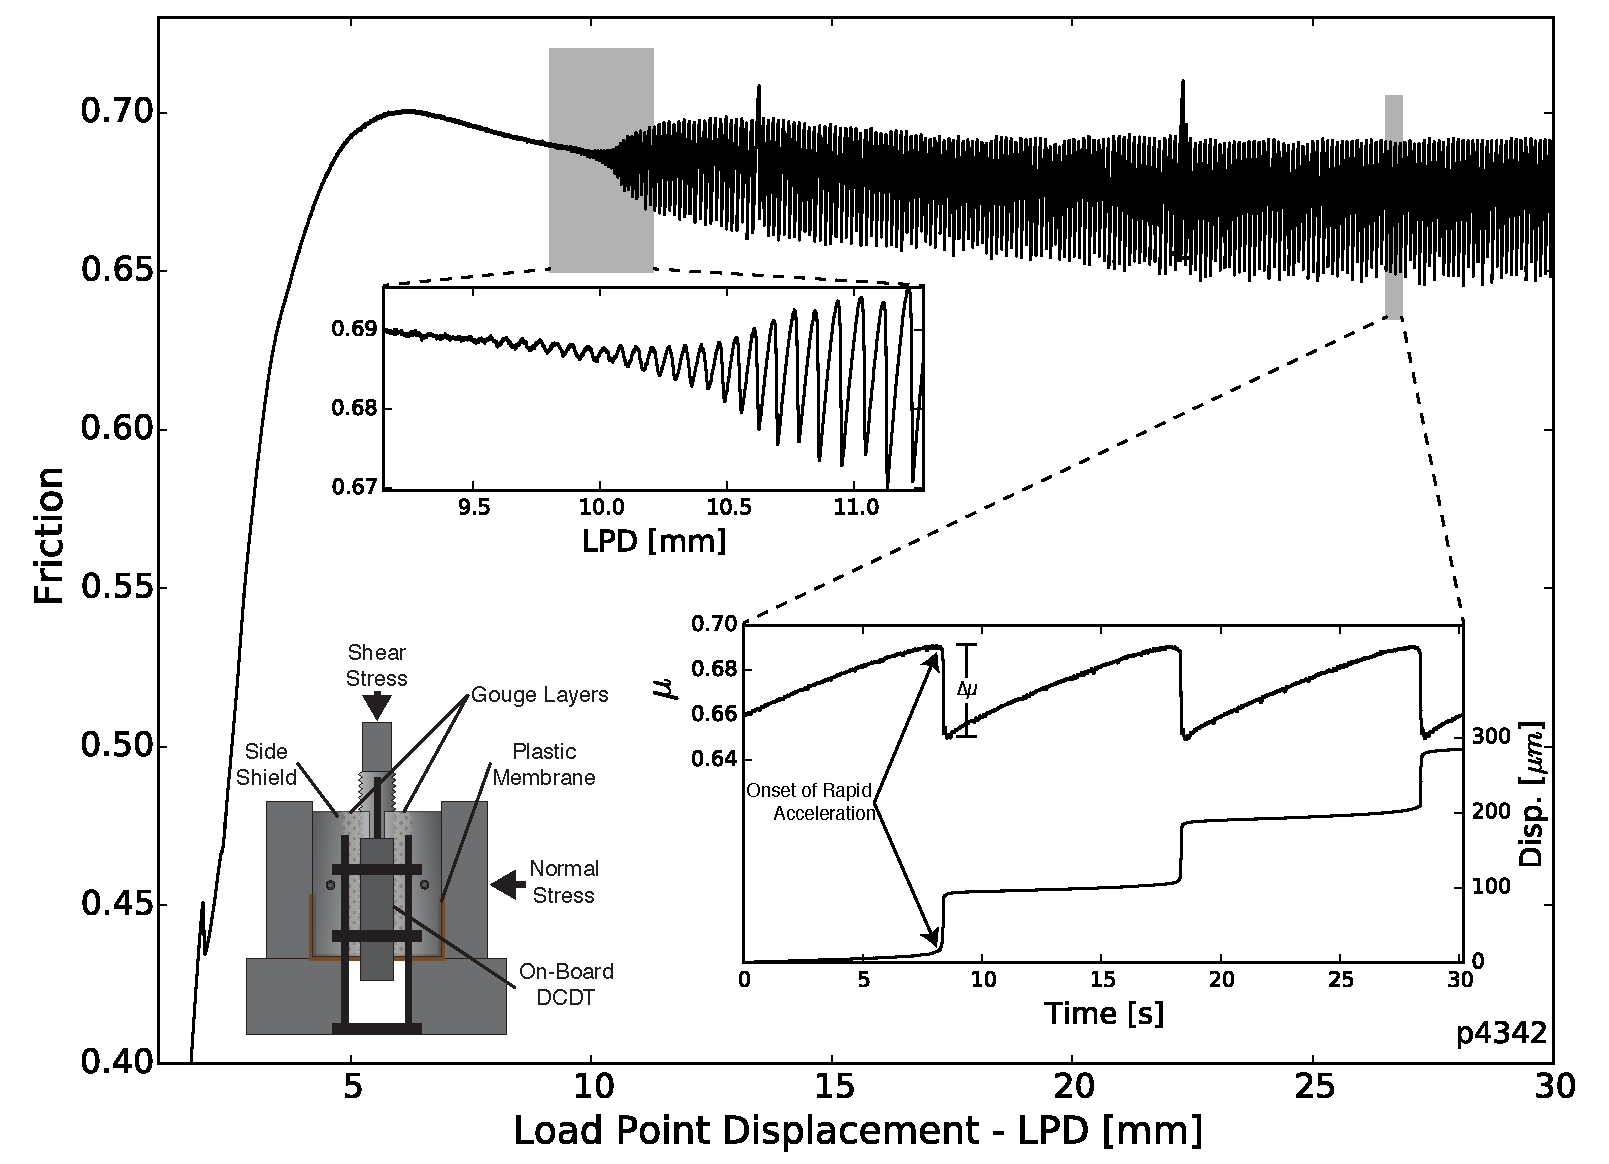
\includegraphics[scale=0.5]{chap_lab_slow_eq/Figure_1.pdf}
   	\caption{Experimental run plot. Friction data for one experiment (p4342) at a normal stress of 12 MPa and shearing rate of 10 $\mu \text{ms}^{-1}$. The upper inset shows spontaneous emergence of unstable slow slip. Stick-slip amplitude increases gradually over a few mm before reaching steady-state.  The lower right inset shows details of fault slip events, note the gradual acceleration at the start of each failure event. The lower left inset shows the double direct shear configuration and locations of displacement transducers. Spikes at 13 mm and 22 mm displacement are due to brief pauses in shearing to reset displacement transducers.}
  	\label{Figure_1}
\end{figure}
% End Figure %

% Figure %
\begin{figure}
	\centering
		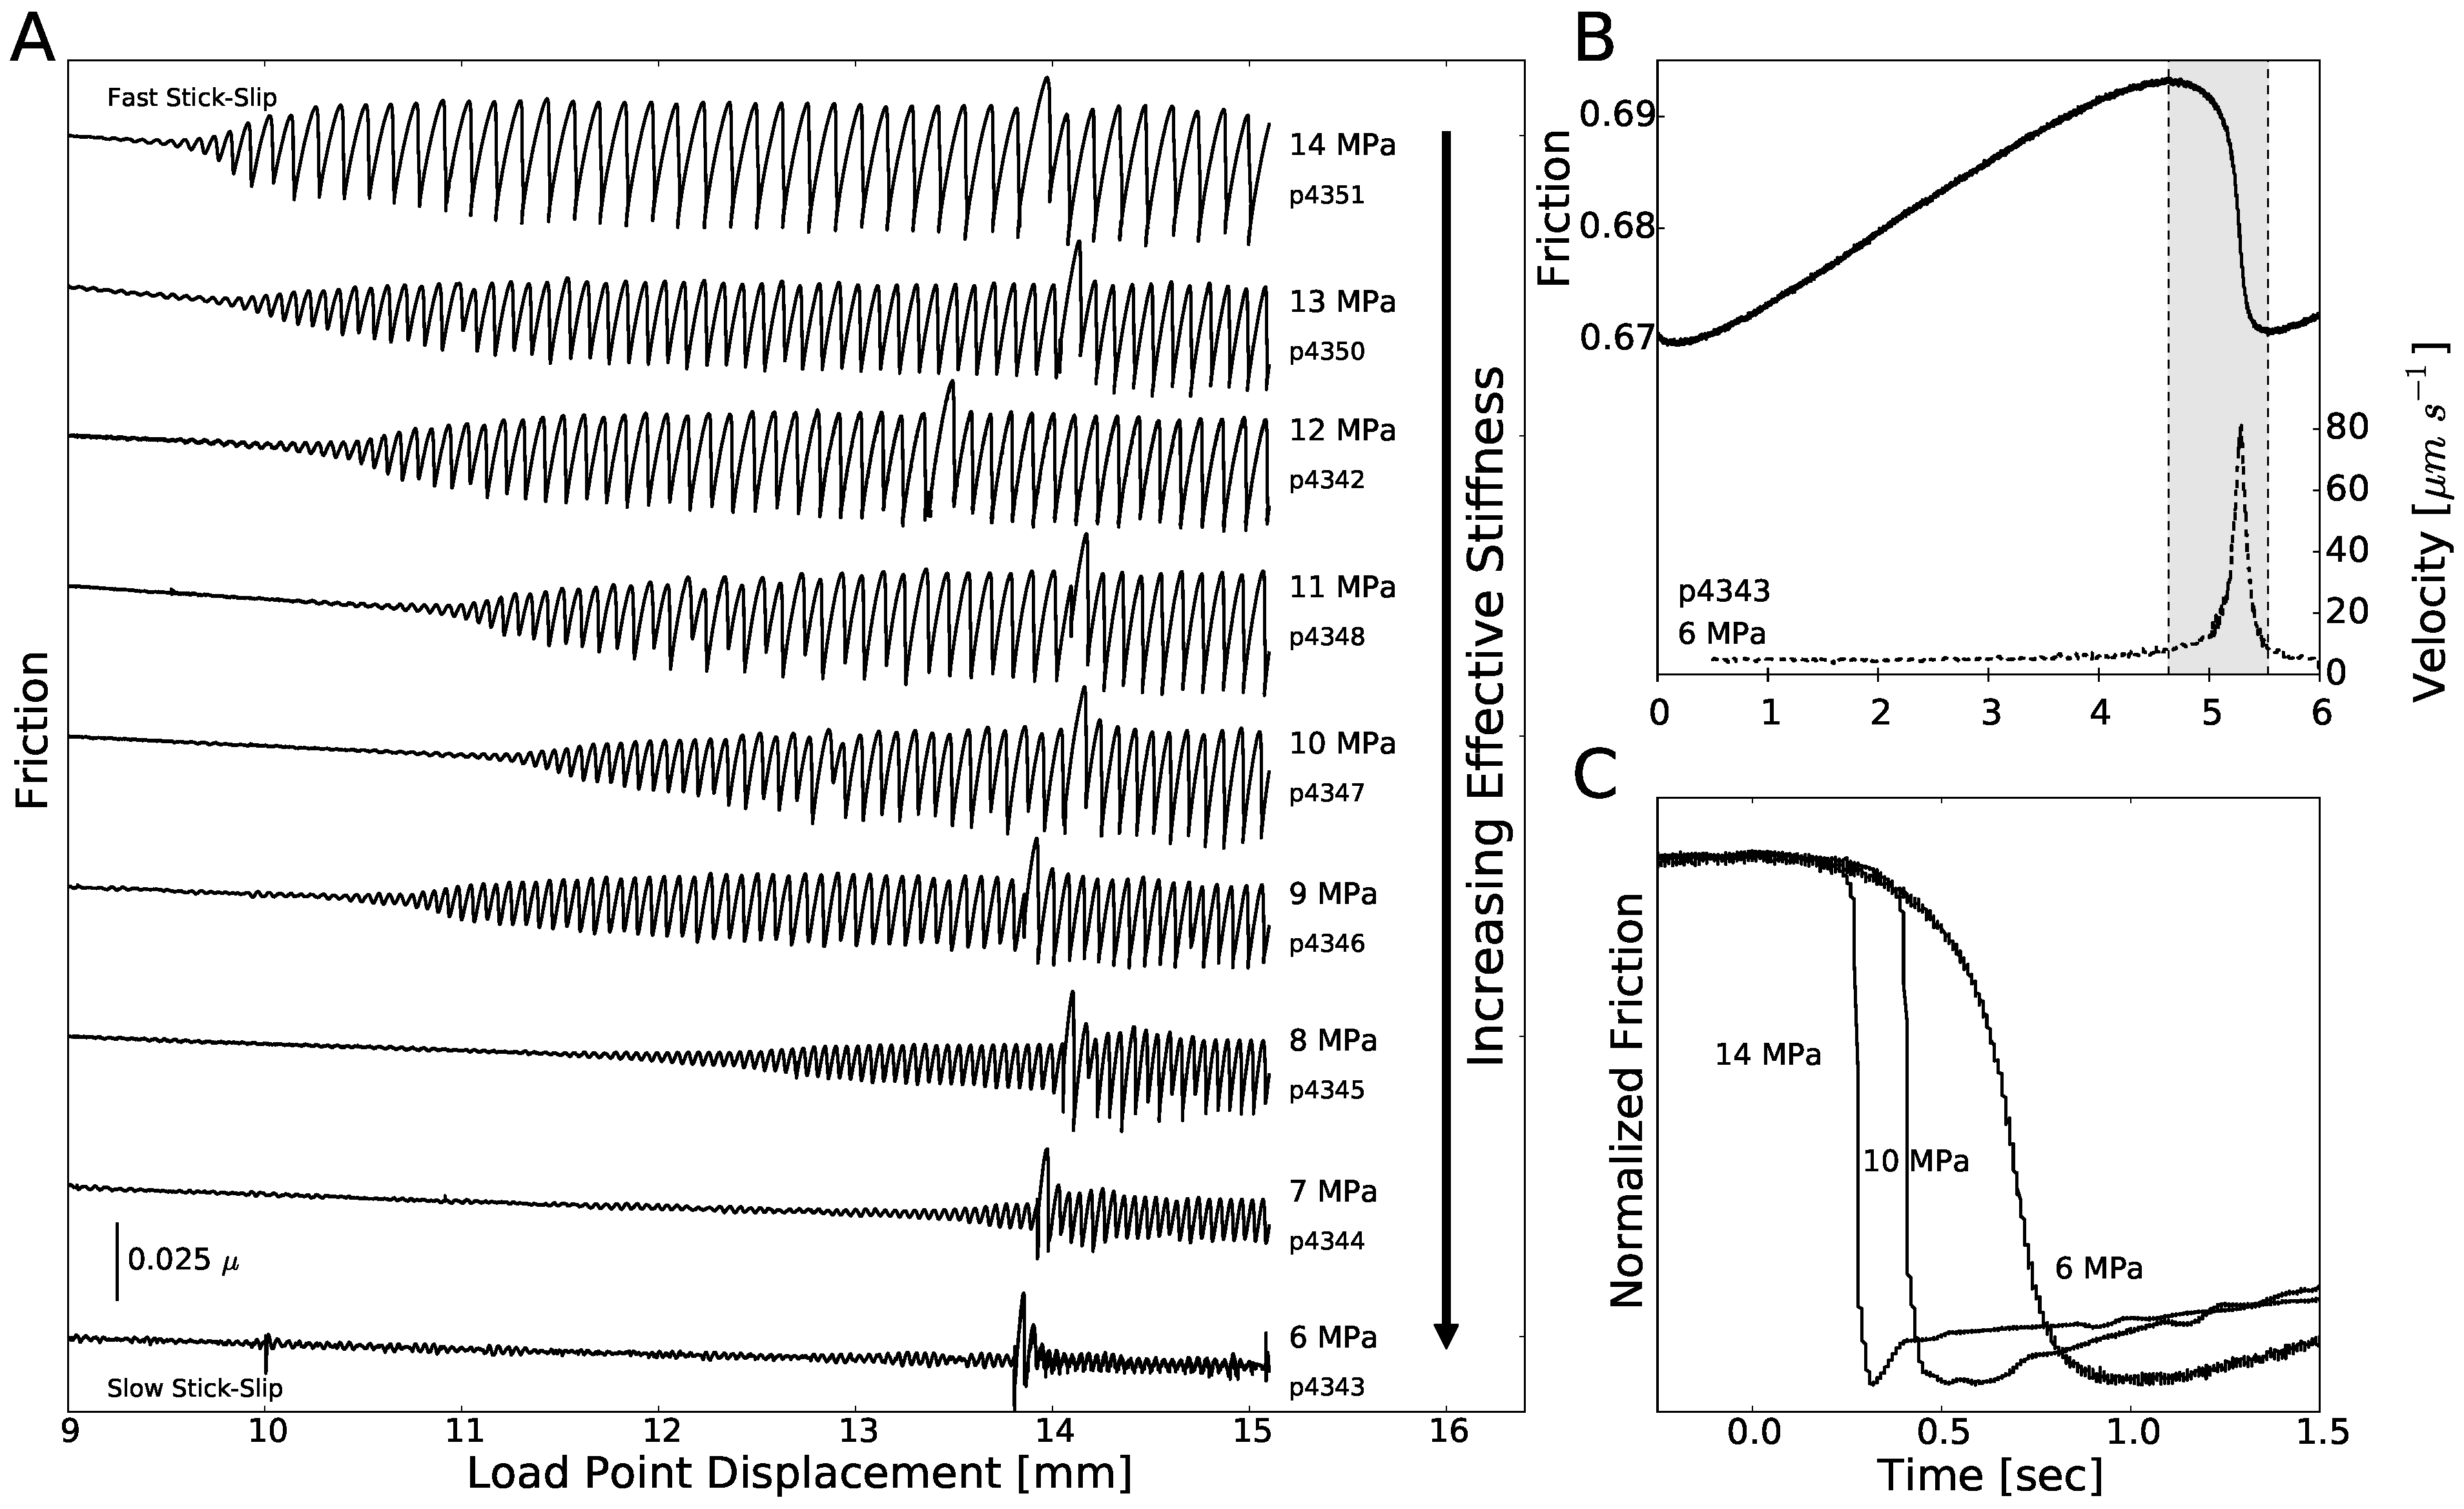
\includegraphics[scale=0.25]{chap_lab_slow_eq/Figure_2.pdf}
   	\caption{Spectrum of Fault Slip Behavior. A) Friction data for experiments (p43XX run numbers) at different effective shear loading stiffness $k'=k/\sigma'_n$. Friction data are offset vertically for clarity. The emergence of slow stick-slip occurs at lower shear displacement, and stick-slip amplitude increases, for higher normal stress experiments. The spikes in friction at 13-15 mm are due to frictional aging caused by brief pauses in shearing to reset displacement transducers. B) Details of friction (solid line) and velocity (dashed) during a stick-slip event with a peak slip velocity of $\sim \mu \text{ms}^{-1}$, only a few times that of the background loading velocity of 10 $\mu \text{ms}^{-1}$. C) Stick-slip events have systematically longer duration at lower normal stresses. Slip accelerates more slowly and event durations are correspondingly longer than at higher normal stress.}
  	\label{Figure_2}
\end{figure}
% End Figure %

% Figure %
\begin{figure}
	\centering
		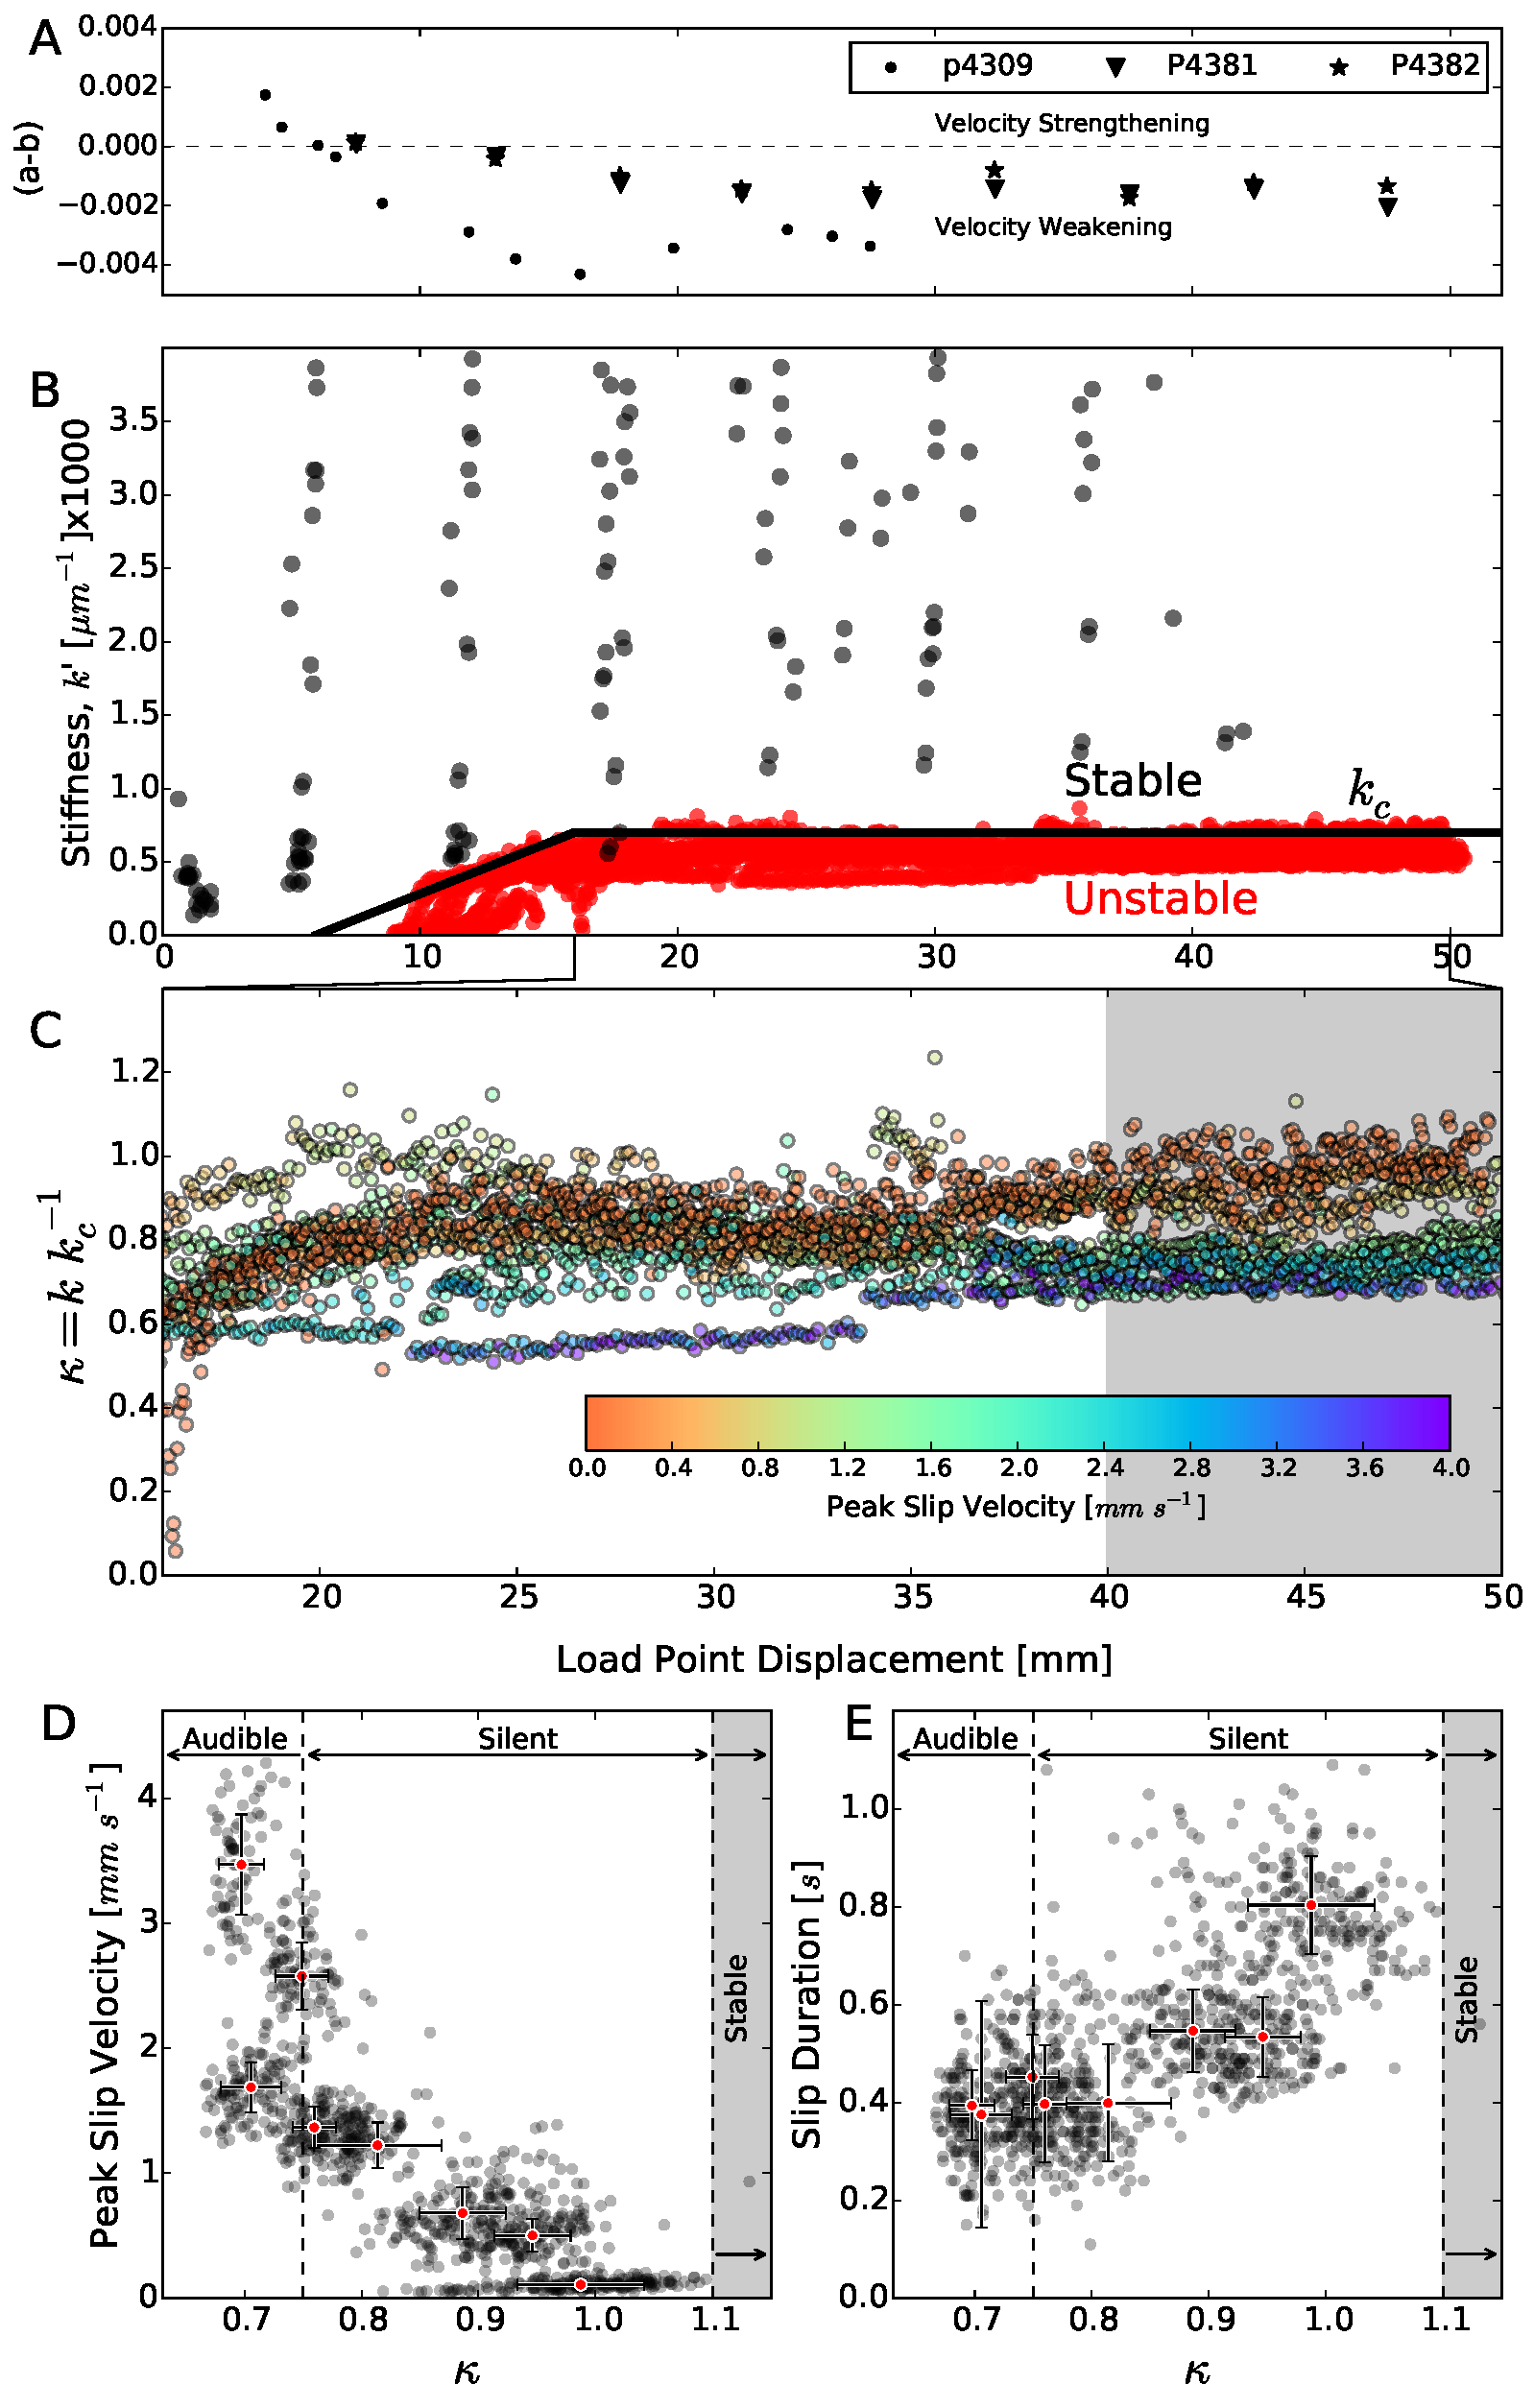
\includegraphics[scale=0.4]{chap_lab_slow_eq/Figure_3.pdf}
   	\caption{Stick slip event properties. A) The friction rate parameter (b-a) transitions from velocity strengthening 
to velocity weakening at $\sim$5-7 mm displacement.  B) Data from 29 experiments showing effective friction stiffness $k'=k/\sigma'_n$ as a function of shear displacement for stable sliding (black dots) and stick-slip events (red dots). The heavy black line defines the evolution of $k'_\text{c}$ based on the distinction between stable sliding and stick-slip. C) Data for unstable slip events shown in B are color coded by peak slip velocity and shown as a function of shear displacement. Stick-slip is slowest for $\kappa \sim 1$. The 40-50 mm interval marked by the gray box denotes data used to compile stick-slip properties. D) Stick-slip event velocity and E) duration as a function of normalized critical stiffness $\kappa = k/k_\text{c}$.  Black dots show data from events in the displacement interval 40-50 mm for 8 experiments; red dots show mean values $\pm 1$ standard deviation for each experiment.}
  	\label{Figure_3}
\end{figure}
% End Figure %

% Figure %
\begin{figure}
	\centering
		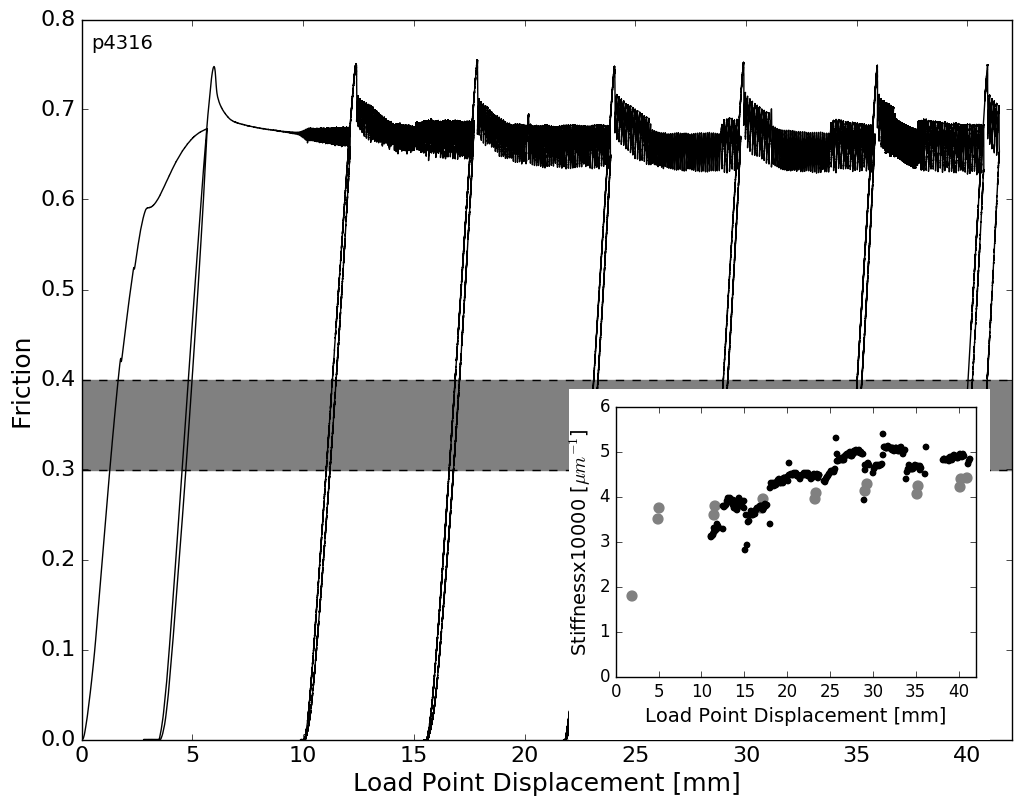
\includegraphics[scale=0.5]{chap_lab_slow_eq/Figure_S1.png}
   	\caption{Stiffness during an experiment. Friction data for one complete experiment (run p4316) with shear load-unload cycles. Slow slip events emerge spontaneously at a displacement of $\sim$8.5 mm. (Inset) Stiffness measured from unload-reload cycles in the range $\mu=0.3-0.4$ (large grey circles) and from the slope of the elastic loading segments of individual stick-slip events (small black circles). Both measurements indicate an initial increase in stiffness, caused by shear enhanced compaction. In this experiment we explored multiple shearing rates during slow slip (e.g., for events in the range 27-29 mm and 31-33 mm), which had a clear effect on stick-slip amplitude and stiffness.}
  	\label{Figure_S1}
\end{figure}
% End Figure %

% Figure %
\begin{figure}
	\centering
		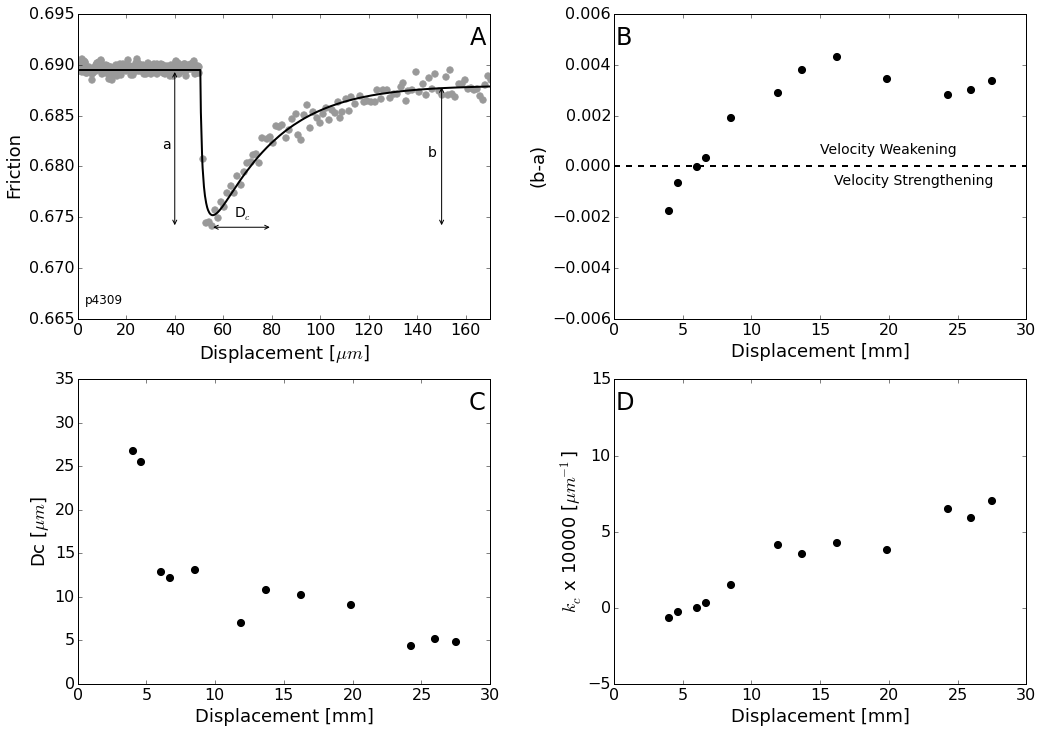
\includegraphics[scale=0.4]{chap_lab_slow_eq/Figure_S2.png}
   	\caption{Rate and State Parameters. Data and modeling procedure for obtaining rate-and-state friction parameters and their variation with shear displacement. A) Data from experiment p4309 (grey data points) and model (solid line) for a velocity step test from 10 to 1 $\mu \text{ms}^{-1}$, with illustration of the friction direct effect a, evolution effect b, and critical slip distance Dc. B) Evolution of (b-a) with shear displacement (see also \ref{Figure_3}A). Note the transition from rate strengthening to rate weakening at $\sim$8 mm displacement, after which a steady-state behavior is reached. C) The critical slip distance decreases with shear displacement as frictional steady-state is reached. D) Evolution of the critical stiffness ($k_\text{c}$) with slip.}
  	\label{Figure_S2}
\end{figure}
% End Figure %

\begin{landscape}

    \begin{longtable}{ |c|c|c|c|c|c| }
    \hline
    Experiment & Blocks & Normal Stress [MPa] & Humidity [\%] & Comments & Unload/Reload Cycles\\
    \hline
    p4224 & Ti/Acrylic & 5 & 16 & Stable - Vel. Steps & N\\
    \hline
    p4228 & Steel& 4 & 100 & Stable - Slide Hold & N\\
    \hline
    p4229 & Ti/Acrylic & 4 & 100 & Failed & N\\
    \hline
    p4248 & Ti/Acrylic & 4 & 100 & Stable - Vel. Steps & N\\
    \hline
    p4249 & Ti/Acrylic & 4 & 100 & Stable - Vel. Steps & N\\
    \hline
    p4267 & Ti/Acrylic & 2 & 100 & Stable - Vel. Steps & Y\\
    \hline
    p4268 & Ti/Acrylic & 8 & 100 & Slow-Slip & Y\\
    \hline
    p4269 & Steel & 4 & 100 & Stable - Vel. Steps & Y\\
    \hline
    p4270 & Steel & 2 & 100 & Stable - Vel. Steps & Y\\
    \hline
    p4271 & Ti/Acrylic & 2 & 100 & Stable - Vel. Steps & Y\\
    \hline
    p4272 & Ti/Acrylic & 8 & 100 & Slow-Slip & Y\\
    \hline
    p4273 & Steel & 8 & 100 & Stable - Vel. Steps & Y\\
    \hline
    p4309 & Steel & 8 & 100 & Stable - Vel. Steps & Y\\
    \hline
    p4310 & Ti/Acrylic & 8 & 100 & Slow-Slip & Y\\
    \hline
    p4311 & Ti/Acrylic & 8 & 100 & Slow-Slip & Y\\
    \hline
    p4312 & Steel/Acrylic & 8 & 100 & Slow-Slip & Y\\
    \hline
    p4313 & Ti/Acrylic & 8 & 100 & Slow-Slip & Y\\
    \hline
    p4314 & Steel & 12 & 100 & Stable - Vel. Steps & Y\\
    \hline
    p4316 & Ti/Acrylic & 12 & 100 & Stick-Slip & Y\\
    \hline
    p4317 & Steel/Acrylic & 12 & 100 & Stick-Slip & Y\\
    \hline
    p4327 & Steel & 6 & 100 & Stable - Vel. Steps & Y\\
    \hline
    p4328 & Ti/Acrylic & 6 & 100 & Slow-Slip & Y\\
    \hline
    p4329 & Ti/Acrylic & 6 & 100 & Slow-Slip & Y\\
    \hline
    p4330 & Steel & 6 & 100 & Stable - Vel. Steps & Y\\
    \hline
    p4338 & Ti/Acrylic & 4 & 100 & Stable - Vel. Steps & Y\\
    \hline
    p4339 & Steel & 4 & 100 & Stable - Vel. Steps & Y\\
    \hline
    p4340 & Ti/Acrylic & 8 & 100 & Slow-Slip & Y\\
    \hline
    p4341 & Steel & 12 & 100 & Stable - Vel. Steps & Y\\
    \hline
    p4342 & Ti/Acrylic & 12 & 100 & Slow/Fast Slip & N\\
    \hline
    p4343 & Steel/Acrylic & 6 & 100 & Slow-Slip & N\\
    \hline
    p4344 & Ti/Acrylic & 7 & 100 & Slow-Slip & N\\
    \hline
    p4345 & Steel/Acrylic & 8 & 100 & Slow-Slip & N\\
    \hline
    p4346 & Ti/Acrylic & 9 & 100 & Slow-Slip & N\\
    \hline
    p4347 & Steel/Acrylic & 10 & 100 & Slow/Fast Slip & N\\
    \hline
    p4348 & Ti/Acrylic & 11 & 100 & Slow/Fast Slip & N\\
    \hline
    p4350 & Steel/Acrylic & 13 & 100 & Slow/Fast Slip & N\\
    \hline
    p4351 & Ti/Acrylic & 14 & 100 & Slow/Fast Slip & N\\
    \hline
    p4381 & Steel & 4 & 100 & Stable - Vel. Steps & N\\
    \hline
    p4382 & Ti & 4 & 100 & Stable - Vel. Steps & N\\
    \hline
\end{longtable}
\end{landscape}
